% The Getting-started vault: a short lab report that explains endleaf as you read it.
% Lines that start with % are comments: LaTeX skips them, and they never reach the PDF.
\documentclass[reprint,aps,pra]{revtex4-2} % pra: the Physical Review A layout
\usepackage{amsmath}  % equations
\usepackage{graphicx} % \includegraphics, for figures
\usepackage{siunitx}  % \qty, for numbers with units
\sisetup{uncertainty-mode = separate} % print 9.75 \pm 0.08, not 9.75(8)

\begin{document}

% The front matter: title, author and affiliation, then the abstract.
\title{Measuring $g$ with a simple pendulum}
\author{A. Student}
\affiliation{Department of Physics}
\date{\today}

\begin{abstract}
We timed a simple pendulum at nine lengths between \qty{0.20}{m} and \qty{1.00}{m}.
The period grows as the square root of the length, and the slope of that
line gives the acceleration due to gravity, $g = \qty{9.75 \pm 0.08}{m/s^2}$,
within one standard error of the standard value. Along the way, this report
shows you how endleaf works.
\end{abstract}

\maketitle

\section{Introduction}

This folder is a \emph{vault}: a folder of related files, here a lab
report. Everything in it stays on your own disk, and the list on the left
shows what's inside. You're reading \texttt{main.tex} in \emph{Live view},
where maths and formatting appear as they will in print, and the line your
cursor is on shows its LaTeX. Press Ctrl+Shift+L to switch to \emph{Source
view}, which shows the plain LaTeX everywhere, and again to come back.

Saving builds the PDF. Press Ctrl+S now: endleaf saves the file, runs LaTeX
on it, and shows the PDF in the pane on the right (Ctrl+Alt+V shows or hides
that pane). Each clean build also leaves a copy in the vault's \texttt{pdf}
folder, ready to hand in. This first build will stop on an error, because this
sentence has a \emhp{deliberate} mistake in it. The Problems panel opens
below with the error explained in plain English. Click the error to jump to
its line, fix the misspelt command, and save again.

The title, author and abstract at the top of this file are the \emph{front
matter}. In \texttt{revtex}, the style of the American Physical Society's
journals, they come before \verb|\maketitle|, which typesets them. Put your
own name in \verb|\author| now.

A simple pendulum is about the plainest experiment in physics, and it still
has something to teach~\cite{nelson1986}. This one measures the acceleration
due to gravity, $g$, from the way the pendulum's period depends on its length.

\section{Theory}

The line above starts a numbered section, and \verb|\subsection| would start
one a level down. The Contents view on the left lists them. A long report
can be split across files: the Methods section below lives in its own file,
\texttt{methods.tex}, and the line \verb|% methods.tex: the Methods section, brought into main.tex by % methods.tex: the Methods section, brought into main.tex by % methods.tex: the Methods section, brought into main.tex by \input{methods}.
% It has no \documentclass or \begin{document}; those belong to main.tex alone.
% Saving here builds main.tex, the document this file belongs to.
\section{Methods}

You're now in \texttt{methods.tex}. A file brought in with \verb|\input| is
part of the same document: its section numbers, equations and citations
carry on from \texttt{main.tex}. Alt+PageUp goes back to the file before it.

A steel bob of mass \qty{52}{g} hung from a light, inextensible string
clamped between two plates. The length $L$, from the clamp to the centre of
the bob, was measured with a metre rule to \qty{\pm 2}{mm}, and set to nine
values from \qty{0.20}{m} to \qty{1.00}{m}.

For each length, the bob was pulled aside by about \ang{10}, small enough
that $\sin\theta \approx \theta$, and released. A handheld stopwatch timed ten
full swings, starting on the third swing so the release didn't count. Each
length was timed three times. The period $T$ is the mean of the three
times divided by ten, with an uncertainty of \qty{0.02}{s} from reaction
time.
.
% It has no \documentclass or \begin{document}; those belong to main.tex alone.
% Saving here builds main.tex, the document this file belongs to.
\section{Methods}

You're now in \texttt{methods.tex}. A file brought in with \verb|\input| is
part of the same document: its section numbers, equations and citations
carry on from \texttt{main.tex}. Alt+PageUp goes back to the file before it.

A steel bob of mass \qty{52}{g} hung from a light, inextensible string
clamped between two plates. The length $L$, from the clamp to the centre of
the bob, was measured with a metre rule to \qty{\pm 2}{mm}, and set to nine
values from \qty{0.20}{m} to \qty{1.00}{m}.

For each length, the bob was pulled aside by about \ang{10}, small enough
that $\sin\theta \approx \theta$, and released. A handheld stopwatch timed ten
full swings, starting on the third swing so the release didn't count. Each
length was timed three times. The period $T$ is the mean of the three
times divided by ten, with an uncertainty of \qty{0.02}{s} from reaction
time.
.
% It has no \documentclass or \begin{document}; those belong to main.tex alone.
% Saving here builds main.tex, the document this file belongs to.
\section{Methods}

You're now in \texttt{methods.tex}. A file brought in with \verb|\input| is
part of the same document: its section numbers, equations and citations
carry on from \texttt{main.tex}. Alt+PageUp goes back to the file before it.

A steel bob of mass \qty{52}{g} hung from a light, inextensible string
clamped between two plates. The length $L$, from the clamp to the centre of
the bob, was measured with a metre rule to \qty{\pm 2}{mm}, and set to nine
values from \qty{0.20}{m} to \qty{1.00}{m}.

For each length, the bob was pulled aside by about \ang{10}, small enough
that $\sin\theta \approx \theta$, and released. A handheld stopwatch timed ten
full swings, starting on the third swing so the release didn't count. Each
length was timed three times. The period $T$ is the mean of the three
times divided by ten, with an uncertainty of \qty{0.02}{s} from reaction
time.
| brings it in where
it should appear. In Live view that line shows as a card; click it to open
the file.

% Ctrl+M wraps a selection in $...$ for inline maths.
Maths in a sentence goes between dollar signs, so \verb|$\theta$| gives
$\theta$. A pendulum of length $L$, swung through a small angle $\theta$, obeys
% Ctrl+Shift+M makes a display, set on a line of its own.
\[
  \frac{d^2\theta}{dt^2} + \frac{g}{L}\,\theta = 0,
\]
which is simple harmonic motion~\cite{belendez2007}. An equation you will
refer to again gets a number, and a \verb|\label| so you can point to it:
% Ctrl+Shift+E inserts an equation environment.
\begin{equation}
  T = 2\pi\sqrt{\frac{L}{g}}.
  \label{eq:period}
\end{equation}
Write \verb|Eq.~\eqref{eq:period}| and LaTeX fills in the number, here
Eq.~\eqref{eq:period}, and keeps it right if equations are added above it.
(The \verb|~| is a space the line won't break at.) For a symbol you can't
remember the name of, open the $\Sigma$ panel on the left: search for it, or
draw it.

By Eq.~\eqref{eq:period}, a plot of $T$ against $\sqrt{L}$ is a straight
line through the origin with slope $2\pi/\sqrt{g}$.

Numbers with units go in \verb|\qty|, from the \texttt{siunitx} package:
\verb|\qty{9.81}{m/s^2}| gives \qty{9.81}{m/s^2}, with upright units and the
right space before them. (Older papers use \verb|\SI{9.81}{m/s^2}|, which is
the same thing in \texttt{siunitx}'s old syntax.) Compare the two ways of
writing the standard value of $g$ in Live view:
$g = 9.8 m/s^2$ typed as maths, and $g = \qty{9.81}{m/s^2}$ written with
\verb|\qty|. Typed as maths, the units come out in italics, as if $m$ and $s$
were variables, and run into the number. Rewrite the first one with
\verb|\qty|, so that it matches the second.

% methods.tex: the Methods section, brought into main.tex by % methods.tex: the Methods section, brought into main.tex by % methods.tex: the Methods section, brought into main.tex by \input{methods}.
% It has no \documentclass or \begin{document}; those belong to main.tex alone.
% Saving here builds main.tex, the document this file belongs to.
\section{Methods}

You're now in \texttt{methods.tex}. A file brought in with \verb|\input| is
part of the same document: its section numbers, equations and citations
carry on from \texttt{main.tex}. Alt+PageUp goes back to the file before it.

A steel bob of mass \qty{52}{g} hung from a light, inextensible string
clamped between two plates. The length $L$, from the clamp to the centre of
the bob, was measured with a metre rule to \qty{\pm 2}{mm}, and set to nine
values from \qty{0.20}{m} to \qty{1.00}{m}.

For each length, the bob was pulled aside by about \ang{10}, small enough
that $\sin\theta \approx \theta$, and released. A handheld stopwatch timed ten
full swings, starting on the third swing so the release didn't count. Each
length was timed three times. The period $T$ is the mean of the three
times divided by ten, with an uncertainty of \qty{0.02}{s} from reaction
time.
.
% It has no \documentclass or \begin{document}; those belong to main.tex alone.
% Saving here builds main.tex, the document this file belongs to.
\section{Methods}

You're now in \texttt{methods.tex}. A file brought in with \verb|\input| is
part of the same document: its section numbers, equations and citations
carry on from \texttt{main.tex}. Alt+PageUp goes back to the file before it.

A steel bob of mass \qty{52}{g} hung from a light, inextensible string
clamped between two plates. The length $L$, from the clamp to the centre of
the bob, was measured with a metre rule to \qty{\pm 2}{mm}, and set to nine
values from \qty{0.20}{m} to \qty{1.00}{m}.

For each length, the bob was pulled aside by about \ang{10}, small enough
that $\sin\theta \approx \theta$, and released. A handheld stopwatch timed ten
full swings, starting on the third swing so the release didn't count. Each
length was timed three times. The period $T$ is the mean of the three
times divided by ten, with an uncertainty of \qty{0.02}{s} from reaction
time.
.
% It has no \documentclass or \begin{document}; those belong to main.tex alone.
% Saving here builds main.tex, the document this file belongs to.
\section{Methods}

You're now in \texttt{methods.tex}. A file brought in with \verb|\input| is
part of the same document: its section numbers, equations and citations
carry on from \texttt{main.tex}. Alt+PageUp goes back to the file before it.

A steel bob of mass \qty{52}{g} hung from a light, inextensible string
clamped between two plates. The length $L$, from the clamp to the centre of
the bob, was measured with a metre rule to \qty{\pm 2}{mm}, and set to nine
values from \qty{0.20}{m} to \qty{1.00}{m}.

For each length, the bob was pulled aside by about \ang{10}, small enough
that $\sin\theta \approx \theta$, and released. A handheld stopwatch timed ten
full swings, starting on the third swing so the release didn't count. Each
length was timed three times. The period $T$ is the mean of the three
times divided by ten, with an uncertainty of \qty{0.02}{s} from reaction
time.


\section{Results}

% Ctrl+Alt+F inserts a figure.
Fig.~\ref{fig:period} shows the period against the square root of the length.
A figure is a picture with a caption: \verb|\includegraphics| brings in the
image file (here \texttt{period.pdf}, in this vault), \verb|\caption| gives it
words, and \verb|\label| lets you refer to it as \verb|Fig.~\ref{fig:period}|.
LaTeX decides where on the page it goes, usually the top of a column.

\begin{figure}
  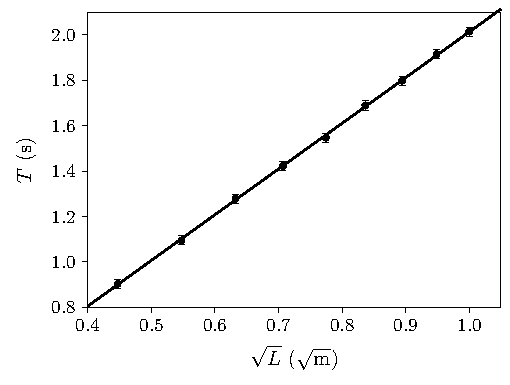
\includegraphics[width=\linewidth]{period.pdf}
  \caption{The period $T$ against $\sqrt{L}$. Error bars are the timing
  uncertainty, \qty{0.02}{s}; the line is a least-squares fit through the
  origin.}
  \label{fig:period}
\end{figure}

The points lie on a straight line, as Eq.~\eqref{eq:period} predicts. Its
slope is \qty{2.013 \pm 0.009}{s.m^{-1/2}}, so
\begin{equation}
  g = \left(\frac{2\pi}{\text{slope}}\right)^2 = \qty{9.75 \pm 0.08}{m/s^2}.
  \label{eq:g}
\end{equation}

\section{Conclusion}

The value in Eq.~\eqref{eq:g} is within one standard error of the standard
acceleration of gravity, \qty{9.80665}{m/s^2}~\cite{nist-gn}. Timing by hand
limits the precision; a light gate would do better.

% Ctrl+Shift+C opens the citation picker.
Citations work like labels. Each source is an entry in
\texttt{references.bib} with a key, and \verb|\cite{nelson1986}| prints its
number and adds it to the References. Only the sources you cite appear there.

To find more, Help \textrightarrow{} Keyboard Shortcuts lists every key, and
Ctrl+Shift+P runs any command by name. To make a lab report of your own,
press Ctrl+N: this vault starts new files from the Lab report template.

\bibliography{references}

\end{document}
